\begin{titlepage}
\thispagestyle{empty}
 \begin{center}
 \begin{figure}[htbp]
    \centering
    \subfloat{
\includegraphics[width=0.4\textwidth]{feulogo}}\hspace{7.5em}
     \subfloat{
\includegraphics[width=0.375\textwidth]{wiwilogo}}\\
 \centering
  \vspace*{1.0cm}
    \subfloat{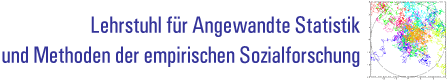
\includegraphics[width=0.75\textwidth]{rechtsfoto}}
\end{figure}

   


  %\vspace*{1.5cm}

  \vspace*{2.5cm}
 {\bf \Large Bewertung von Optionen und zustandsbedingten Anspr{\"u}chen (contingent claims) mit der Feynman-Kac-Formel}
 \vspace*{3.5cm} \\
 {\Large Seminararbeit\\von\\}
 \vspace{0.5cm}
 {\large \bfseries Corvin Idler\\}
c/o European Commission, Delegation Australia, Diplomatic Pouch, \\1049 Brussels, BELGIUM\\
 +61 2 6271 2777, idler@uni-koblenz.de
 \vfill



\begin{table}[h]
	\centering
	\begin{tabular}{|l| l|}\hline
		Studiengang & Bachelor Wirtschaftswissenschaften\\ \hline
		Betreuer & Prof. Dr. Hermann Singer\\ \hline
		Matrikelnummer & 7529953\\ \hline
		Arbeit vorgelegt am: & 22.10.2010\\ \hline
	\end{tabular}
\end{table}

 \end{center}
\end{titlepage}